---
id: tkz-euclide-ejemplo-05
title: Múltiples Puntos
description: "Define varios puntos de una sola vez y los dibuja con sus etiquetas."
keywords: [puntos, multiples, etiquetas]
tags: [tkzDefPoints,tkzDrawPoints,tkzLabelPoints]
sort: 5
---
\documentclass[tikz,border=2mm]{standalone}
\usepackage{tkz-euclide}

\begin{document}
    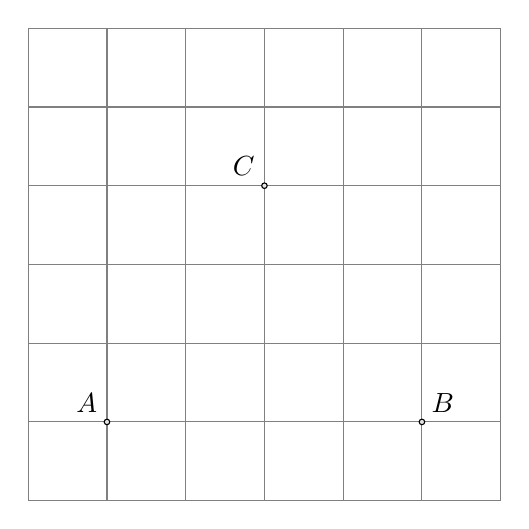
\begin{tikzpicture}
        % Define el sistema de coordenadas ortogonales.
        \tkzInit[xmin=0,xmax=6,ymin=0,ymax=6]
        % Dibuja los ejes del plano cartesiano.
        \tkzDrawXY
        % Dibuja una cuadrícula en el área definida.
        \tkzGrid
    
        % Define un conjunto de puntos.
        \tkzDefPoints{
            1/1/A,
            5/1/B,
            3/4/C%
        }
    
        % Dibuja los puntos definidos como A,B,C.
        \tkzDrawPoints(A,B,C)
        % Etiqueta los puntos A,C arriba a la izquierda.
        \tkzLabelPoints[above left](A,C)
        % Etiqueta los puntos A,C arriba a la derecha.
        \tkzLabelPoints[above right](B)
    \end{tikzpicture}
\end{document}